\chapter{Graphical Models}\label{ch:pgm}

\Cref{part:prediction} was about prediction: given an input $x$, estimate a response $y$, through $f(x)$ or the conditional distribution $p(y\given x)$. \Cref{part:probabilistic} asks a broader question. We model the \emph{joint distribution} $p(x_1,\dots,x_N)$ of many variables, some observed and some hidden, and then answer any query about it: the distribution of one variable given others, the most likely configuration of the hidden variables, or new samples that look like the data. Prediction becomes a special case, conditioning on $x$ to obtain $p(y\given x)$. The difficulty is size: a general joint distribution of $N$ binary variables has $2^N-1$ free parameters. Graphical models make the problem manageable by encoding \emph{conditional independences} in a graph, which makes the representation compact (this chapter), the computation of queries feasible (\cref{ch:inference,ch:mcmc,ch:vi}), and learning from data possible (\cref{ch:latent}). \Cref{sec:pgm-joint} reviews conditional independence; \cref{sec:dag,sec:dsep} treat directed models and how to read independences from them; \cref{sec:mrf,sec:ising} treat undirected models; and \cref{sec:pgm-sequences} applies both ideas to sequences, ending with hidden Markov models.

\section{Joint Distributions and Conditional Independence}\label{sec:pgm-joint}

By the chain rule of probability, every joint distribution factorizes as
\[
p(x_1,\dots,x_N)=\prod_{j=1}^Np(x_j\given x_1,\dots,x_{j-1}),
\]
for any ordering of the variables. This factorization is general and therefore saves nothing: for binary variables the $j$-th factor needs $2^{j-1}$ parameters, and the total is $2^N-1$. Savings come from dropping variables from the conditioning sets, which is justified by conditional independence. For $A\subseteq\{1,\dots,N\}$ write $x_A=\{x_i:i\in A\}$.

\begin{definition}[Conditional Independence]\label{def:cond-indep}
For disjoint index sets $A,B,C$, the variables $x_A$ and $x_B$ are \emph{conditionally independent given} $x_C$, written $x_A\indep x_B\given x_C$, if
\[
p(x_A,x_B\given x_C)=p(x_A\given x_C)\,p(x_B\given x_C),
\]
or equivalently $p(x_A\given x_B,x_C)=p(x_A\given x_C)$, or $p(x_B\given x_A,x_C)=p(x_B\given x_C)$: once $x_C$ is known, learning $x_B$ tells us nothing more about $x_A$.
\end{definition}

\section{Directed Graphical Models}\label{sec:dag}

\begin{definition}[Directed Graphical Model]\label{def:dagm}
Let $G$ be a directed acyclic graph (DAG) whose nodes are the variables $x_1,\dots,x_N$, and let $\mathrm{pa}(i)$ be the set of nodes with an edge into $x_i$. A distribution \emph{factorizes according to} $G$ if
\[
p(x_1,\dots,x_N)=\prod_{i=1}^Np\big(x_i\given x_{\mathrm{pa}(i)}\big).
\]
The pair of $G$ and the conditional distributions is a \emph{directed graphical model}, or \emph{Bayesian network}.
\end{definition}

Comparing with the chain rule, ordered so that parents precede children, a DAG asserts that each variable depends on its predecessors only through its parents. For the graph in \cref{fig:dag6},
\[
p(x_1,\dots,x_6)=p(x_1)\,p(x_2\given x_1)\,p(x_3\given x_1)\,p(x_4\given x_2)\,p(x_5\given x_3)\,p(x_6\given x_2,x_5).
\]
For discrete variables each factor is a \emph{conditional probability table} (CPT). A binary node with $K_i$ parents needs $2^{K_i}$ parameters, one probability for each configuration of its parents, so a DAG needs about $N\,2^{\max_iK_i}$ parameters instead of $2^N-1$. The saving is exponential when every node has few parents.

\begin{figure}[ht]
\centering
\begin{tikzpicture}[
  var/.style={draw, circle, minimum size=7mm, inner sep=0pt, font=\small},
  arr/.style={-{Stealth[length=1.8mm]}, thin}
]
\node[var] (x1) at (0,0) {$x_1$};
\node[var] (x2) at (1.8,0.9) {$x_2$};
\node[var] (x3) at (1.8,-0.9) {$x_3$};
\node[var] (x4) at (3.6,1.5) {$x_4$};
\node[var] (x5) at (3.6,-0.9) {$x_5$};
\node[var] (x6) at (5.4,0.3) {$x_6$};
\draw[arr] (x1) -- (x2); \draw[arr] (x1) -- (x3);
\draw[arr] (x2) -- (x4); \draw[arr] (x3) -- (x5);
\draw[arr] (x2) -- (x6); \draw[arr] (x5) -- (x6);
\end{tikzpicture}
\caption{The running example of a DAG from the lectures.}
\label{fig:dag6}
\end{figure}

\subsection{Example: Naive Bayes}

The tutorial classifies texts as spam ($C=1$) or not ($C=0$) from binary indicators $X_1,\dots,X_d$ of which dictionary words appear. Applying the chain rule in the order $C,X_1,\dots,X_d$ gives a fully connected DAG with $1+\sum_{i=1}^d2^i=2^{d+1}-1$ parameters, as many as the unrestricted joint distribution. The \emph{naive Bayes} model deletes every edge between words and keeps only the edges $C\to X_i$ (\cref{fig:nb-hmm}, left):
\[
p(C,X_1,\dots,X_d)=p(C)\prod_{i=1}^dp(X_i\given C),
\]
which says that the words are conditionally independent given the class. With $p(C=1)=\pi$ and $p(X_j=1\given C=c)=\theta_{j,c}$ the model has $1+2d$ parameters, linear rather than exponential in $d$, and maximum likelihood (\cref{sec:mle}) gives frequencies:
\[
\hat\pi=\frac{\#\{\text{spam texts}\}}{n},\qquad \hat\theta_{j,c}=\frac{\#\{\text{texts of class $c$ containing word $j$}\}}{\#\{\text{texts of class $c$}\}}.
\]
The posterior $p(C\given X)\propto p(C)\prod_ip(X_i\given C)$ then classifies new texts. This is the naive Bayes classifier of \cref{sec:naive-bayes}, now read off a graph.

\begin{figure}[ht]
\centering
\begin{tikzpicture}[
  var/.style={draw, circle, minimum size=7.5mm, inner sep=0pt, font=\small},
  obs/.style={var, fill=black!15},
  arr/.style={-{Stealth[length=1.8mm]}, thin}
]
\begin{scope}
\node[var] (c) at (1.5,1.2) {$C$};
\node[obs] (a) at (0,0) {$X_1$};
\node[obs] (b) at (1,0) {$X_2$};
\node at (2,0) {$\cdots$};
\node[obs] (d) at (3,0) {$X_d$};
\draw[arr] (c) -- (a); \draw[arr] (c) -- (b); \draw[arr] (c) -- (d);
\end{scope}
\begin{scope}[xshift=5.2cm]
\node[var] (z1) at (0,1.2) {$z_1$};
\node[var] (z2) at (1.4,1.2) {$z_2$};
\node[var] (z3) at (2.8,1.2) {$z_3$};
\node (zd) at (4.0,1.2) {$\cdots$};
\node[obs] (o1) at (0,0) {$x_1$};
\node[obs] (o2) at (1.4,0) {$x_2$};
\node[obs] (o3) at (2.8,0) {$x_3$};
\draw[arr] (z1) -- (z2); \draw[arr] (z2) -- (z3); \draw[arr] (z3) -- (zd);
\draw[arr] (z1) -- (o1); \draw[arr] (z2) -- (o2); \draw[arr] (z3) -- (o3);
\end{scope}
\end{tikzpicture}
\caption{Left: naive Bayes. Right: a hidden Markov model (\cref{sec:hmm}). Shaded nodes are observed.}
\label{fig:nb-hmm}
\end{figure}

\section{Reading Independences from a DAG: d-Separation}\label{sec:dsep}

A DAG implies many conditional independences beyond the ones used to define it. All of them can be read off the graph by examining three elementary configurations of three nodes (\cref{fig:triples}).

\begin{figure}[ht]
\centering
\begin{tikzpicture}[
  var/.style={draw, circle, minimum size=7mm, inner sep=0pt, font=\small},
  arr/.style={-{Stealth[length=1.8mm]}, thin},
  lab/.style={font=\small\itshape, align=center}
]
\begin{scope}
\node[var] (x) at (0,0) {$x$};
\node[var] (y) at (1.3,0) {$y$};
\node[var] (z) at (2.6,0) {$z$};
\draw[arr] (x) -- (y); \draw[arr] (y) -- (z);
\node[lab] at (1.3,-1.0) {(a) causal chain};
\end{scope}
\begin{scope}[xshift=4.4cm]
\node[var] (y) at (1.0,0.7) {$y$};
\node[var] (x) at (0,-0.3) {$x$};
\node[var] (z) at (2.0,-0.3) {$z$};
\draw[arr] (y) -- (x); \draw[arr] (y) -- (z);
\node[lab] at (1.0,-1.0) {(b) common cause};
\end{scope}
\begin{scope}[xshift=8.4cm]
\node[var] (x) at (0,0.7) {$x$};
\node[var] (z) at (2.0,0.7) {$z$};
\node[var] (y) at (1.0,-0.3) {$y$};
\draw[arr] (x) -- (y); \draw[arr] (z) -- (y);
\node[lab] at (1.0,-1.0) {(c) common effect};
\end{scope}
\end{tikzpicture}
\caption{The three canonical triples. In (a) and (b), observing $y$ blocks the flow of information between $x$ and $z$; in (c), observing $y$ (or one of its descendants) opens it.}
\label{fig:triples}
\end{figure}

\begin{enumerate}[(a)]
  \item \emph{Causal chain} $x\to y\to z$: $p(x,y,z)=p(x)p(y\given x)p(z\given y)$, so $p(z\given x,y)=p(z\given y)$ and $x\indep z\given y$. Without conditioning, $x$ and $z$ are in general dependent.
  \item \emph{Common cause} $x\leftarrow y\to z$: $p(x,z\given y)=p(y)p(x\given y)p(z\given y)/p(y)=p(x\given y)p(z\given y)$, so again $x\indep z\given y$. Two effects of a common cause are correlated until the cause is known.
  \item \emph{Common effect} $x\to y\leftarrow z$: $p(x,y,z)=p(x)p(z)p(y\given x,z)$, so $x\indep z$ marginally, but in general $x\not\indep z\given y$. This is \emph{explaining away}: if an alarm $y$ can be set off by a burglary $x$ or an earthquake $z$, then given that the alarm rang, learning that there was an earthquake makes a burglary less likely.
\end{enumerate}

Call a triple $u\text{--}v\text{--}w$ on a path \emph{active} given the observed set $C$ if information can flow through $v$: for a chain or a common cause, if $v\notin C$; for a common effect $u\to v\leftarrow w$, if $v$ or one of its descendants is in $C$. Otherwise the triple is \emph{blocked}.

\begin{definition}[d-Separation]\label{def:dsep}
A path between two nodes is \emph{active} given $C$ if every consecutive triple along it is active. Sets $A$ and $B$ are \emph{d-separated} by $C$ if no path from a node of $A$ to a node of $B$ is active given $C$.
\end{definition}

\begin{theorem}[d-Separation and Conditional Independence]\label{thm:dsep}
If $A$ and $B$ are d-separated by $C$ in $G$, then $x_A\indep x_B\given x_C$ for every distribution that factorizes according to $G$. Conversely, if they are not d-separated, then there is some distribution factorizing according to $G$ in which $x_A$ and $x_B$ are dependent given $x_C$.
\end{theorem}

\begin{remark}[What ``Vice Versa'' Means]
The slides state that d-separation implies conditional independence ``and vice versa''. The converse holds only in the sense of the theorem: a particular distribution may have extra independences, for instance because its CPT entries happen to cancel, that the graph does not show. d-Separation lists exactly the independences that hold for \emph{all} distributions compatible with the graph.
\end{remark}

The lectures check d-separation with the \emph{Bayes ball} procedure: shade the observed nodes, then try to travel from $A$ to $B$, passing through a node only when the triple formed there is active. If $x_C$ is clamped and we ``wiggle'' $x_A$, the question is whether any node in $B$ can move.

\begin{algorithm}[H]
\caption{Checking $x_A\indep x_B\given x_C$ by d-Separation (Bayes Ball)}\label{alg:dsep}
\begin{algorithmic}[1]
\Input{A DAG $G$, disjoint node sets $A$, $B$, $C$.}
\Init{Shade the nodes in $C$; mark every node that is in $C$ or has a descendant in $C$.}
\For{each $a\in A$}
  \State Explore, by depth-first search, the paths that start at $a$ and do not revisit a node; the first step may go to any neighbor of $a$ along an edge in either direction.
  \State Extend a path $\dots,u,v$ to a neighbor $w$ of $v$ only if the triple $u\text{--}v\text{--}w$ is active:
  \Statex \hspace{2.6em} chain or common cause at $v$: $v$ is not shaded;
  \Statex \hspace{2.6em} common effect $u\to v\leftarrow w$: $v$ is marked.
  \If{some path reaches a node of $B$}
    \State \Return ``$x_A\not\indep x_B\given x_C$ in general''
  \EndIf
\EndFor
\Output{``$x_A\indep x_B\given x_C$'' (no active path exists).}
\end{algorithmic}
\end{algorithm}

In \cref{fig:dag6}, is $x_1\indep x_6\given\{x_2,x_3\}$? The paths from $x_1$ to $x_6$ are $x_1\to x_2\to x_6$, blocked by the shaded chain node $x_2$, and $x_1\to x_3\to x_5\to x_6$, blocked at $x_3$. So the answer is yes. Is $x_2\indep x_3\given\{x_1,x_6\}$? The path $x_2\to x_6\leftarrow x_5\leftarrow x_3$ is active: $x_6$ is an observed common effect and $x_5$ an unobserved chain node. So the answer is no, even though the other path $x_2\leftarrow x_1\to x_3$ is blocked.

Two consequences of d-separation are used repeatedly. Every node is conditionally independent of its non-descendants given its parents. And the \emph{Markov blanket} of $x_i$, the smallest set that makes $x_i$ independent of all other nodes, consists of its parents, its children, and the other parents of its children. The co-parents enter because of explaining away, and in large DAGs they can make the blanket look unintuitive: nodes far from $x_i$ in the picture belong to it while closer ones do not. For some problems, moreover, there is no natural direction for the edges. Both observations motivate undirected models.

\section{Markov Random Fields}\label{sec:mrf}

In an undirected graphical model, or \emph{Markov random field} (MRF), edges represent symmetric interactions between neighboring variables rather than conditional distributions. A \emph{clique} is a set of nodes that are all pairwise connected; a \emph{maximal clique} cannot be enlarged by adding another node.

\begin{definition}[Markov Random Field]\label{def:mrf}
Let $G$ be an undirected graph on $x=(x_1,\dots,x_N)$ with set of maximal cliques $\cC$. A distribution \emph{factorizes according to} $G$ if
\[
p(x)=\frac1Z\prod_{C\in\cC}\psi_C(x_C),\qquad Z=\sum_x\prod_{C\in\cC}\psi_C(x_C),
\]
for some nonnegative \emph{potential functions} $\psi_C$. The normalizing constant $Z$ is the \emph{partition function} (an integral for continuous variables).
\end{definition}

Potentials are not probabilities: they are arbitrary nonnegative scores, large for compatible configurations of the clique, and only the product is normalized. For discrete variables a potential is a table of nonnegative numbers. The price of this freedom is $Z$, a sum over all configurations, whose computation is in general as hard as inference itself.

\begin{theorem}[Hammersley--Clifford]\label{thm:hammersley-clifford}
If $p(x)>0$ for all $x$, the following are equivalent:
\begin{enumerate}[(i)]
  \item $p$ factorizes according to $G$;
  \item $p$ satisfies the \emph{global Markov property}: $x_A\indep x_B\given x_S$ whenever $S$ separates $A$ from $B$ in $G$, that is, every path from $A$ to $B$ passes through $S$.
\end{enumerate}
In particular, if $x_i$ and $x_j$ are not adjacent then $x_i\indep x_j\given x_{\text{rest}}$, and the Markov blanket of $x_i$ is the set of its neighbors.
\end{theorem}

Reading independences off an MRF is simpler than in a DAG: it is plain graph separation, with no special case for common effects. For the graph in \cref{fig:mrf7}, the maximal cliques give
\[
p(x)\propto\psi_{123}(x_1,x_2,x_3)\,\psi_{235}(x_2,x_3,x_5)\,\psi_{245}(x_2,x_4,x_5)\,\psi_{356}(x_3,x_5,x_6)\,\psi_{4567}(x_4,x_5,x_6,x_7),
\]
and separation yields, for example, $(x_1,x_2)\indep(x_6,x_7)\given(x_3,x_4,x_5)$ and $x_1\indep x_5\given(x_2,x_3)$.

\begin{figure}[ht]
\centering
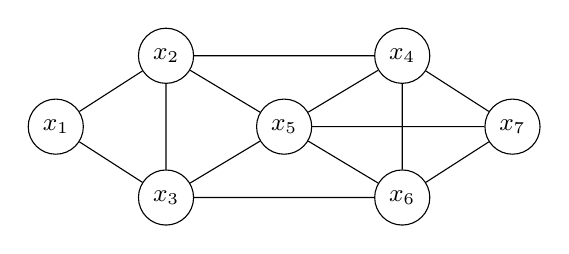
\begin{tikzpicture}[
  var/.style={draw, circle, minimum size=7mm, inner sep=0pt, font=\small}
]
\node[var] (1) at (0,0) {$x_1$};
\node[var] (2) at (1.4,0.9) {$x_2$};
\node[var] (3) at (1.4,-0.9) {$x_3$};
\node[var] (5) at (2.9,0) {$x_5$};
\node[var] (4) at (4.4,0.9) {$x_4$};
\node[var] (6) at (4.4,-0.9) {$x_6$};
\node[var] (7) at (5.8,0) {$x_7$};
\draw (1)--(2) (1)--(3) (2)--(3) (2)--(5) (3)--(5) (2)--(4) (4)--(5) (3)--(6) (5)--(6) (4)--(6) (4)--(7) (5)--(7) (6)--(7);
\end{tikzpicture}
\caption{The MRF example of the lectures, with maximal cliques $\{1,2,3\}$, $\{2,3,5\}$, $\{2,4,5\}$, $\{3,5,6\}$, $\{4,5,6,7\}$.}
\label{fig:mrf7}
\end{figure}

Directed and undirected models express different families of independences, and neither contains the other. The four-cycle $A\text{--}B\text{--}C\text{--}D\text{--}A$ has the two independences $A\indep C\given\{B,D\}$ and $B\indep D\given\{A,C\}$, and no DAG on four nodes has exactly these. Conversely, the common effect $x\to y\leftarrow z$ has $x\indep z$ but $x\not\indep z\given y$; an undirected graph that connects $x$ and $z$ through $y$ cannot make them marginally independent while keeping them dependent given $y$.

\begin{remark}[Connection to Exponential Families]
Write each potential in log-linear form, $\log\psi_C(x_C\given\theta_C)=\theta_C\T\phi_C(x_C)$. Then
\[
p(x\given\theta)=\exp\Big\{\sum_{C\in\cC}\theta_C\T\phi_C(x_C)-A(\theta)\Big\},\qquad A(\theta)=\log Z(\theta),
\]
an exponential family (\cref{sec:expfam}) with sufficient statistics $\phi_C$. For discrete variables this is no restriction: let $\phi_C(x_C)$ be the indicator vector of the configuration $x_C$ and $\theta_C$ the table of log-potentials. The usual exponential-family identity gives $\partial A/\partial\theta_C=\E[\phi_C(X_C)]$: derivatives of the log-partition function are marginal probabilities of the cliques. This is one reason why computing marginals (\cref{ch:inference}) is the central computational task for MRFs.
\end{remark}

\section{The Ising Model and Gaussian Graphical Models}\label{sec:ising}

The \emph{Ising model}, originally a model of magnetism, is the prototypical MRF. The variables are spins $x_s\in\{-1,+1\}$ on the nodes of a graph, often a grid. Each edge $s\sim t$ carries a pairwise potential $\psi_{st}(x_s,x_t)=e^{J_{st}x_sx_t}$, equal to $e^{J_{st}}$ when the spins agree and $e^{-J_{st}}$ when they disagree, and each node may carry a field $\psi_s(x_s)=e^{b_sx_s}$. Together,
\[
p(x)\propto\exp\Big\{\sum_{s\sim t}J_{st}\,x_sx_t+\sum_sb_s\,x_s\Big\}.
\]
A coupling $J_{st}>0$ favors equal neighboring spins, and by \cref{thm:hammersley-clifford} $J_{st}=0$ means $x_s\indep x_t\given x_{\text{rest}}$. In an image, the spins are black or white pixels and positive couplings express that neighboring pixels tend to agree. This model reappears throughout \cref{part:probabilistic}: for image denoising with loopy belief propagation (\cref{sec:loopy-bp}), with Gibbs sampling (\cref{alg:gibbs}), and with mean-field variational inference (\cref{sec:mean-field}).

The continuous analogue is the multivariate Gaussian (\cref{sec:gaussian}). With precision matrix $K=\Sigma^{-1}$,
\[
p(x)\propto\prod_s\exp\Big\{-\tfrac12K_{ss}(x_s-\mu_s)^2\Big\}\prod_{s<t}\exp\big\{-K_{st}(x_s-\mu_s)(x_t-\mu_t)\big\},
\]
a pairwise MRF in which $-K_{st}$ plays the role of the coupling $J_{st}$. Hence $K_{ij}=0$ if and only if $x_i\indep x_j\given x_{\text{rest}}$: the graph of a \emph{Gaussian graphical model} is the sparsity pattern of the precision matrix, not of the covariance matrix. A zero covariance $\Sigma_{ij}=0$ instead means marginal independence.

\section{Models for Sequences}\label{sec:pgm-sequences}

Much data comes in sequences: time series such as prices or speech, and ordered data such as text or genes. The i.i.d.\ assumption of \cref{part:prediction} no longer applies, and the chain rule $p(x_{1:T})=\prod_tp(x_t\given x_{1:t-1})$ needs factors with ever longer histories. The simplest remedy is a Markov assumption.

\subsection{Markov Chains}

A \emph{first-order Markov chain} assumes $p(x_t\given x_{1:t-1})=p(x_t\given x_{t-1})$, so
\[
p(x_{1:T})=p(x_1)\prod_{t=2}^Tp(x_t\given x_{t-1}),
\]
the DAG $x_1\to x_2\to\dots\to x_T$. The chain is \emph{time-homogeneous} (the slides call it stationary) if $p(x_{t+1}=j\given x_t=i)$ does not depend on $t$. An $m$-th order chain conditions on $x_{t-m:t-1}$; this is useful for language, where dependencies reach further back. For $x_t\in\{1,\dots,K\}$ the transitions form a $K\times K$ \emph{transition matrix} $A$ with $A_{ij}=p(x_t=j\given x_{t-1}=i)$ and rows summing to one, drawn as a state transition diagram whose arrows are the nonzero entries. The marginal distribution evolves as $p(x_t=j)=\sum_iA_{ij}\,p(x_{t-1}=i)$, and the $n$-step transition probabilities are the entries of $A^n$ (the Chapman--Kolmogorov equations, $A(m+n)=A(m)A(n)$). The long-run behavior of $A^n$, the stationary distribution, is the basis of Markov chain Monte Carlo and is studied in \cref{sec:markov-chains}.

A first-order chain over words is a simple \emph{language model}. Its parameters, the initial distribution $\pi_j=p(x_1=j)$ and the matrix $A$, are estimated by maximum likelihood from sentences treated as independent, and the log-likelihood $\sum_jN_j^1\log\pi_j+\sum_{j,k}N_{jk}\log A_{jk}$ depends on the data only through counts.

\begin{algorithm}[H]
\caption{Maximum Likelihood for a Markov Chain (Bigram Language Model)}\label{alg:markov-mle}
\begin{algorithmic}[1]
\Input{Sequences $x^{(1)},\dots,x^{(N)}$ over states $\{1,\dots,K\}$, of lengths $T_1,\dots,T_N$.}
\State $N_j^1\gets\sum_{i=1}^N\ind\{x^{(i)}_1=j\}$ for each $j$ \Comment{how often state $j$ starts a sequence}
\State $N_{jk}\gets\sum_{i=1}^N\sum_{t=1}^{T_i-1}\ind\{x^{(i)}_t=j,\ x^{(i)}_{t+1}=k\}$ for each $j,k$ \Comment{transition counts}
\Output{$\hat\pi_j=N_j^1/\sum_{j'}N_{j'}^1$ and $\hat A_{jk}=N_{jk}/\sum_{k'}N_{jk'}$.}
\end{algorithmic}
\end{algorithm}

The estimates are the empirical frequencies of starting states and of transitions out of each state, just as the naive Bayes estimates above are empirical frequencies: whenever every factor of a directed model is a free categorical distribution and all variables are observed, maximum likelihood decouples into one counting problem per CPT.

\subsection{Hidden Markov Models}\label{sec:hmm}

In many applications the quantity that evolves in a Markovian way is not observed directly. A \emph{hidden Markov model} (HMM) has hidden states $z_t\in\{1,\dots,K\}$ that form a Markov chain and observations $x_t$, in any space, that depend only on the current state (\cref{fig:nb-hmm}, right):
\[
p(x_{1:T},z_{1:T})=p(z_1)\prod_{t=2}^Tp(z_t\given z_{t-1})\prod_{t=1}^Tp(x_t\given z_t).
\]
By d-separation, $z_t$ separates the past from the future, but the observations alone are not Markov: every path from $x_{t-2}$ to $x_t$ runs through unobserved states, so all past observations remain informative. An HMM is thus a latent variable model, like the mixtures of \cref{ch:latent}, with the mixture components linked over time. Computing $p(z_t\given x_{1:T})$ is an inference problem on a chain, solved by the message passing of \cref{ch:inference}.

Graphs can also be designed from domain knowledge rather than generic assumptions. The QMR network for medical diagnosis is bipartite, with about 570 hidden diseases pointing to about 4000 observed symptoms through ``noisy-OR'' CPTs; the ALARM network for monitoring intensive-care patients has 37 discrete variables but, being sparse, only 504 parameters instead of at least $2^{37}-1$ (its variables have up to four states).

\begin{notebox}{Pros and Cons}
Graphical models give a compact and interpretable representation of a high-dimensional distribution: the graph states the modeling assumptions, the number of parameters scales with the size of the largest family or clique rather than with $2^N$, and conditional independences can be read off by d-separation or graph separation. DAGs are natural when there is a causal or generative story and are easy to sample from; MRFs are natural for symmetric interactions such as neighboring pixels. However, the graph only describes structure. Computing with the model, through marginals, conditionals, or the partition function, can still be very expensive, and an MRF's potentials are hard to interpret and to learn because of $Z$.
\end{notebox}

\begin{notebox}{Limitations and what comes next}
A graphical model defines $p(x)$, but the questions we care about, such as $p(x_A\given x_B)$, require summing the joint distribution over all configurations of the remaining variables, which is exponential in their number if done naively. \Cref{ch:inference} shows how to exploit the factorization to compute such sums exactly by variable elimination and message passing, and when this remains too expensive, \cref{ch:mcmc,ch:vi} approximate them by sampling and by optimization.
\end{notebox}
